\chapter{Google Dialogflow}

Dialogflow\cite{dialogflow} is a platform developed by Google to build natural and rich conversational experiences. Much like the Microsoft's Botframework, Dialogflow aims to make it possible for chatbot creators to create a single chatbot that connects to multiple channels like Skype, Slack and Messenger, etc.

Dialogflow seems to focus on the usage of their GUI and tools to create conversations, but it's also possible to write all of the logic using code.

\section{Business Model}

Google offers 2 main pricing options for their platform. Firstly there is the free edition, it includes free usage with unlimited text query requests. These requests are limited to 3 queries per second. It's also possible to easily integrate voice interaction into Dialogflow, the free edition limits these kinds of interactions to 1000 requests per day with a maximum of 15000 per month. Support is also limited to community and email support. Google themselves recommend this plan for small to medium businesses or developers trying to experiment with Dialogflow. Next to the free edition, there is an enterprise edition as well. This edition has a pay as you go model, which means it's easily scalable as the business will be paying per request. Choosing this option also opens up the possibility to integrate Google Cloud Support and receive specialized instant support.

\section{Technical implementation}

Because Dialogflow is very focused on their GUI, small to medium businesses that don't need extensive logic in their chatbot can make use of the existing tools to create a chatbot. This is recommended to get started and get familiar with the platform. When more complicated logic needs to be implemented like API calls and custom logic that wouldn't be supported by the platform, custom \Gls{Webhook}s can be created. These allow developers to receive a message that was recognized by Dialogflow and implement their custom logic to handle the message.

It's also possible to take full advantage of Dialogflow using their client libraries. These libraries are available for C\#, GO, Java, Node.JS, PHP, Python and Ruby. There is some documentation available to get started but diving deeper into the development will take great effort. To take advantage of this functionality, the enterprise edition of Dialogflow needs to be used.

\subsection{Developer environment}

There are several ways to choose a development environment and set up a workflow. Using Google Dialogflow isn't just focused on coding, developers mostly need to work with the user interface provided by google.

To get started, simply making use of the website GUI will suffice. There is also an inline editor~\ref{fig:dialogflow-inline-editor} provided to handle requests in code. Another way to handle requests is by enabling a custom webhook to receive information from Dialogflow, like an intent that was recognized, and handle it. This webhook would be written by the developer, following Dialogflow's specification to send back messages. Setting up this webhook is completely up to the developer, it can be done in any server language and does not make use of any library linked to Dialogflow, all the webhook will receive is a simple POST request.

\begin{figure}[ht]
	\centering
	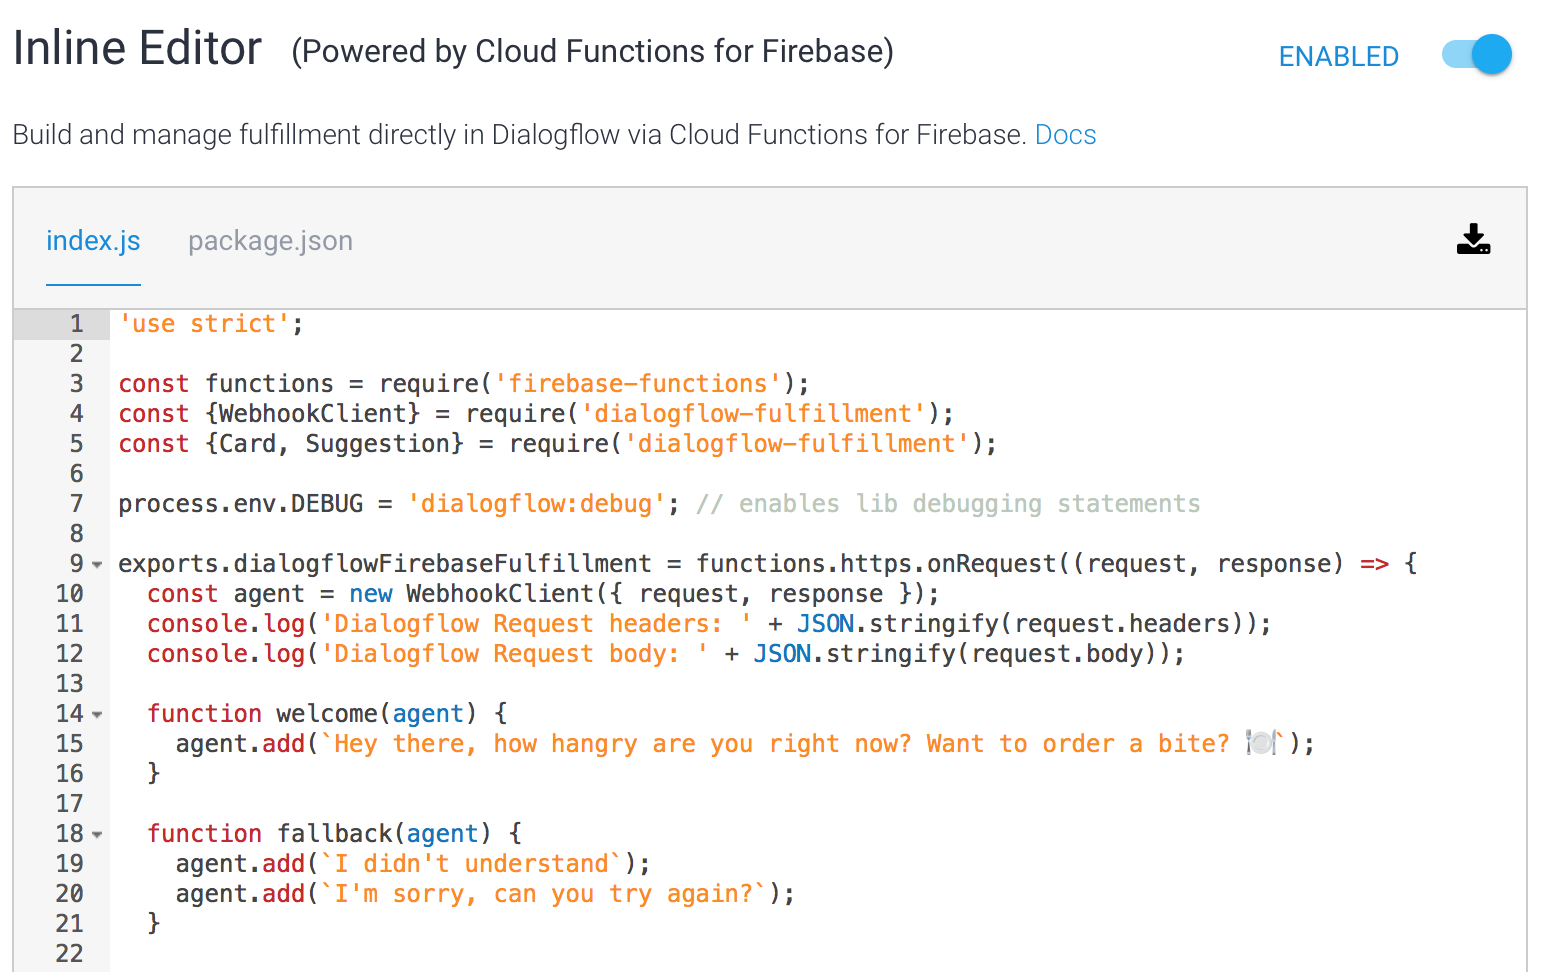
\includegraphics[width=0.8\textwidth]{dialogflow-inline-editor}\label{fig:dialogflow-inline-editor}
	\caption{Dialogflow's inline editor for handling intents}
\end{figure}

\subsection{Testing}

\begin{wrapfigure}{r}{0.35\textwidth}
	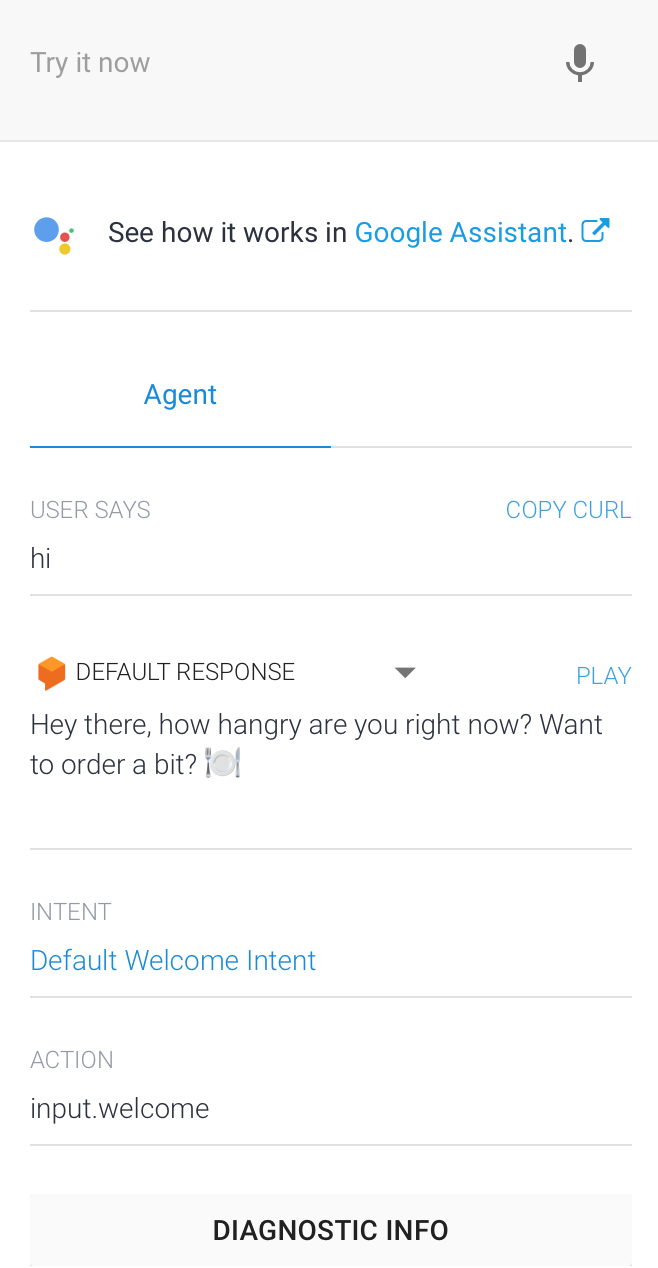
\includegraphics[width=0.7\linewidth]{dialogflow-testing}\label{fig:dialogflow-testing}
	\caption{Testing a bot using the Dialogflow platform}
\end{wrapfigure}

Testing the bot is done using Dialogflow's own testing segment on the interface. When making use of a custom webhook testing becomes more complicated as the webhook will have to be deployed every time the developer wants to actually test the replies of the chatbot.

\clearpage
\newpage

\section{Building a bot}

\subsection{Initialization}

Because a Dialogflow bot cannot be locally tested using any emulator, initialization of the bot happens on the platform itself. The platform uses a different term for chatbot called `agent'. The agent contains intents, entities and responses towards the user. To begin, a new agent should be created.

This can be done from scratch, or by using one of the prebuilt agents (figure~\ref{fig:dialogflow-prebuilt-agents}) provided by the Dialogflow team as a base. There is a number of prebuilt agents available ranging from simple use cases like setting an alarm to more complicated ones like banking operations or online shopping.

\begin{figure}[ht]
	\centering
	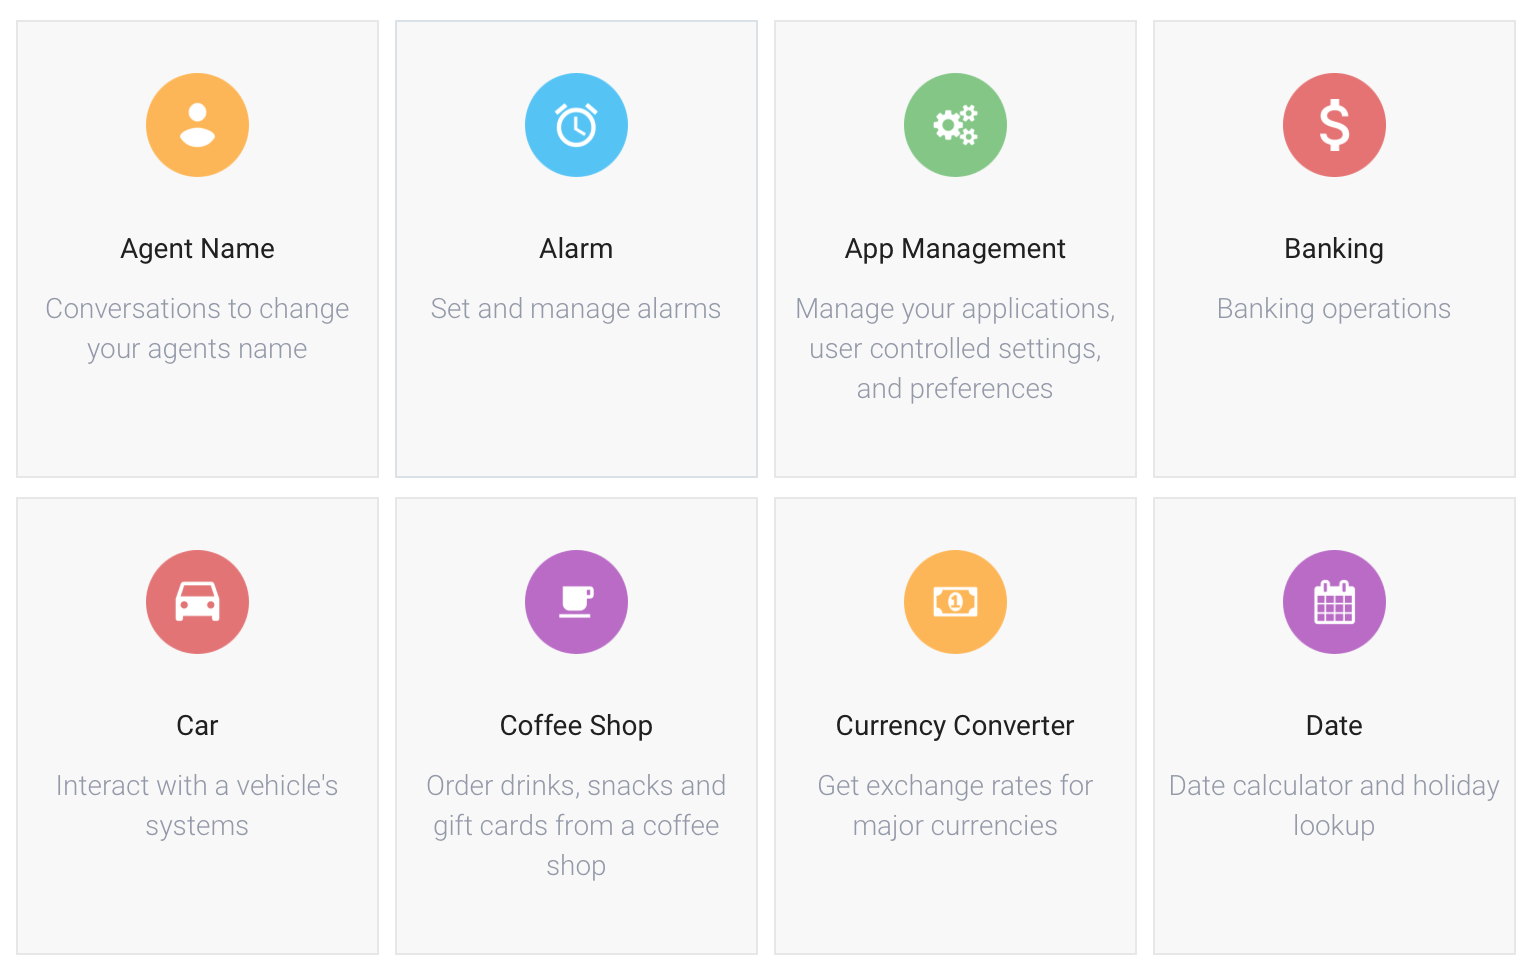
\includegraphics[width=0.9\textwidth]{dialogflow-prebuilt-agents}\label{fig:dialogflow-prebuilt-agents}
	\caption{Some of the prebuilt agents made available by the Dialogflow team}
\end{figure}

Agents are fully customizable and easy to import but the prebuilt agents do not contain any responses. There is also a small talk agent that can be added on top of a main agent to push specific branding and provide users with a more human experience.

\subsection{Intents}

After initialization, intents should be defined. An intent links what the user says to a specific action the bot should take. It represents what a user means and how the agent should react.

Next to a regular intent, a follow-up intent can also be added. These intents follow up on existing intents and are used to for example go through the process of ordering food.

Fallback intents can be defined as well, these will be triggered if none of the user's input matched any of the intents. Typically these are used to define responses like `I didn't get that'. It's where the agent ends up when it doesn't know what to do.

Another useful feature is the ability to add weight to different intents using something called `Intent priority'. This comes in handy when multiple intents were matched but some should be more important than the others.

An intent contains 4 main segments: training phrases, action, response and contexts.

\subsubsection{Training phrases}

A training phrase is an example phrase the user says. Inside of an intent, multiple training phrases can be defined. Dialogflow will recognize a user's response and use these training phrases to link it to a certain intent.

Two types of training phrases can be defined, examples or templates. Examples are the best way of constructing a training phrase. They are written in natural language and certain words are annotated for extraction. Annotation means linking a word to an entity, more on entities later on. Dialogflow can automatically annotate words in the training phrase and recognize certain values like for example a time definition. A template training phrase contains direct references to an entity instead of an annotation.

\begin{figure}[ht]
	\centering
	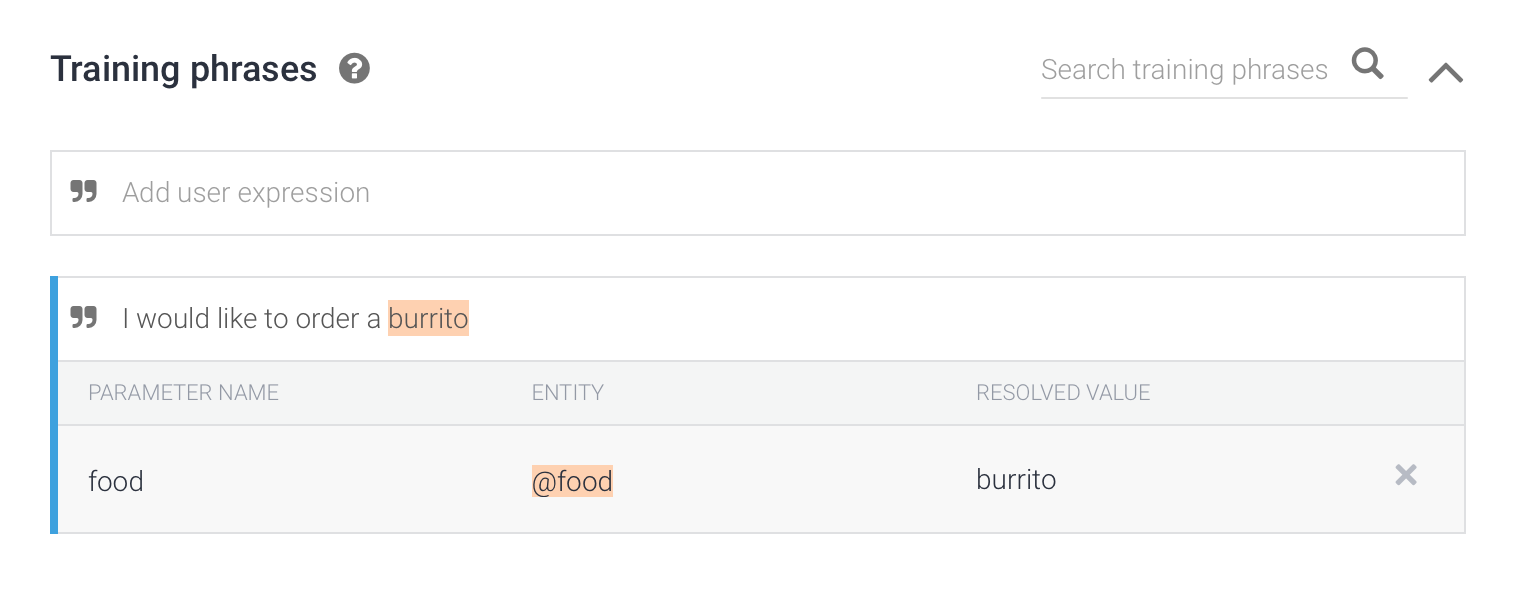
\includegraphics[width=0.9\textwidth]{dialogflow-training-phrases}\label{fig:dialogflow-training-phrases}
	\caption{An example training phrase with an annotated parameter}
\end{figure}

\subsubsection{Action and parameters}

This section contains a single action and its parameters. An action is a simple trigger word for the agent to handle the intent using its recognized parameters. The parameter table is connected to the training phrases. If some words were automatically annotated and recognized as a parameter from inside the training phrases section, they will have been added to the table. There can be cases where parameters would have to be added manually, which can be done using this section.

\subsubsection{Responses}

This is the section where the bot responses will be defined. Multiple responses can be defined for an intent to allow for variation. Different response types can be added for specific platforms.

\subsubsection{Contexts}

Contexts are parameters that can be passed out of the intent. It's a way for the agent to remember the response of a certain intent and use that response again in a different intent. An example is when a user asks to turn on a specific light somewhere, and in his next message simply sends `Turn it off'. Without context there is no way to determine what the user wants to turn off, but using context the agent can remember that the user was talking about that specific light. These contexts have a default lifespan that can be changed manually as well.

\subsection{Entities}

Entities are a second important part of Dialogflow's toolset. They are used to distinguish important values from a user's input. An example of an entity can be a date, an object or a location.

\begin{figure}[ht]
	\centering
	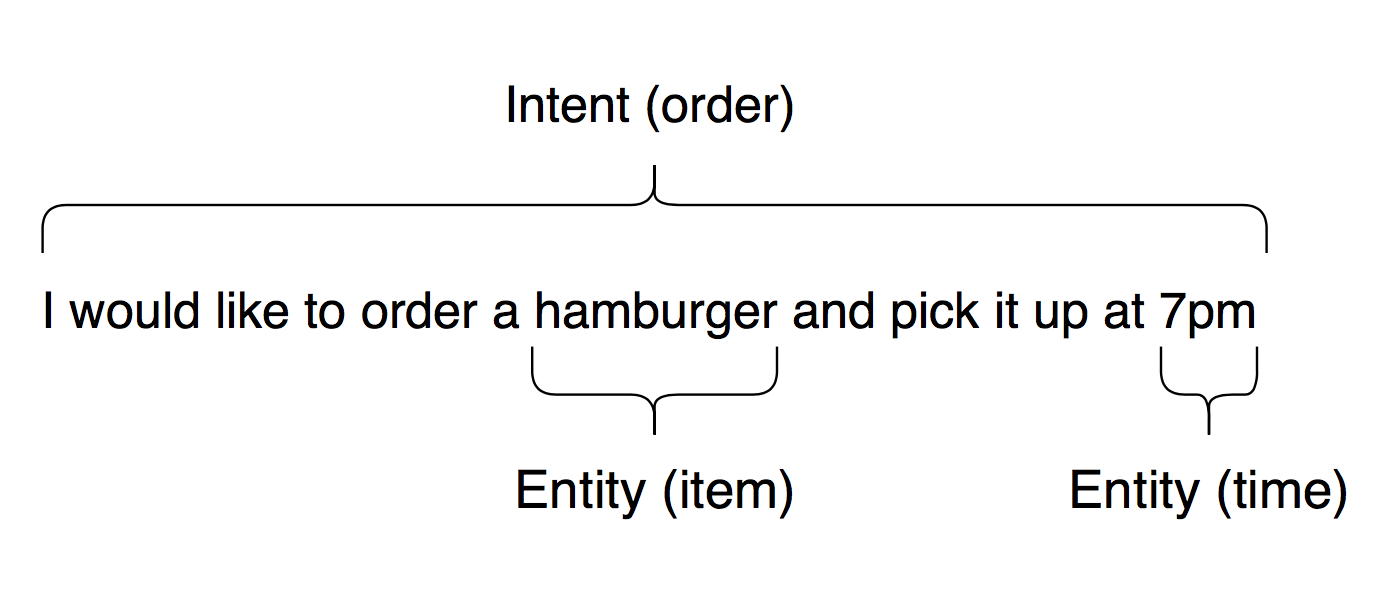
\includegraphics[width=0.9\textwidth]{intent-entity}\label{fig:intent-entity}
	\caption{Representation of an intent and entity}
\end{figure}

There are 3 types of entities in the Dialogflow platform: system, developer and user. These 3 types can each also be divided into a mapping, enum or composite.

\subsubsection{System entities}

System entities are prebuilt entities provided by the Dialogflow platform. They are general entities that can be used everywhere. Examples are the `@sys.date' entity, the `@sys.color' entity or the `@sys.unit-currency' entity. The date entity is an example of a mapping. They match different values like `The first of January' or `01-01-2018' and they map to a specific date format. The color entity on the other hand is an example of an enum. The color gets matched but it doesn't link to a reference value and just returns the color as is. Lastly the unit-currency entity is an example of a composite. It's an entity containing another entity. For example 50 dollars will return an object consisting of 2 values linked to an attribute: the amount will be 50 and the currency will be dollar.

\subsubsection{Developer entities}

It's possible to define custom entities as well. These should be used when the system entities don't cover all of the agents needs.

\subsubsection{User entities}

User entities are entities that are defined on a session level. They entities that can be specifically defined to a user. The use case for this is out of the scope of this thesis and documentation about it is scarce.

\subsubsection{Using entities}

Defining entities or using system entities is pretty straight forward (\ref{fig:entity-creation}). In the case of a food ordering chatbot you could have a custom entity called `food-type'. This kind of entity could be an enum. A food type for the food ordering chatbot would be `starter'.

\begin{figure}[ht]
	\centering
	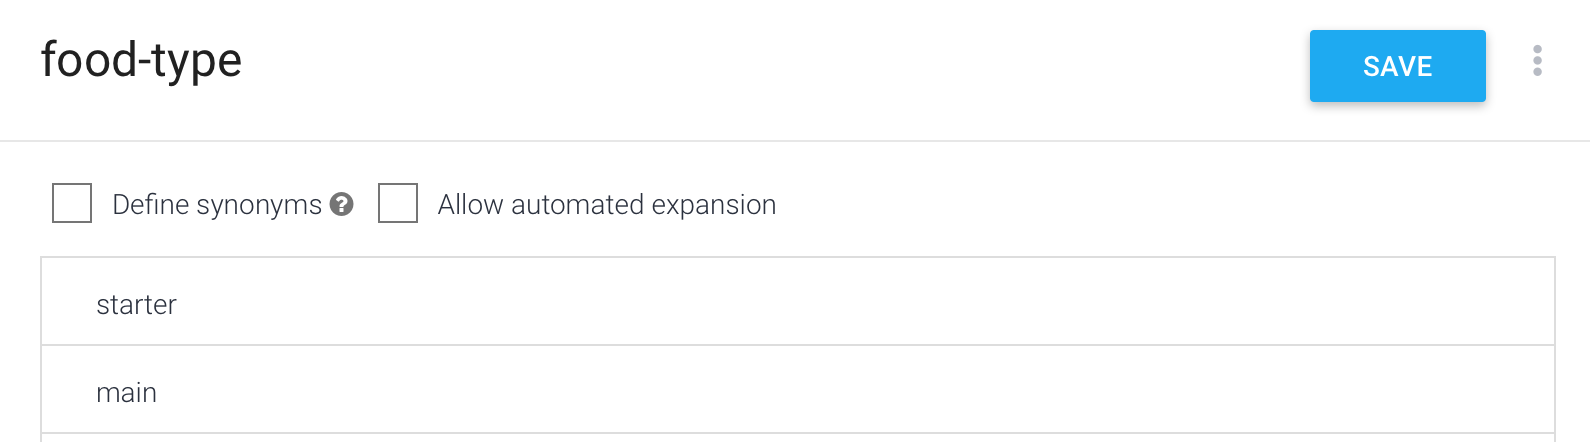
\includegraphics[width=0.9\textwidth]{entity-creation}\label{fig:entity-creation}
	\caption{Creating an enum entity}
\end{figure}

This entity can then be used straight away in any intent by inputting training phrases. The entity will be recognized automatically and added to the parameter table as seen in figure~\ref{fig:parameter-table}.

\begin{figure}[ht]
	\centering
	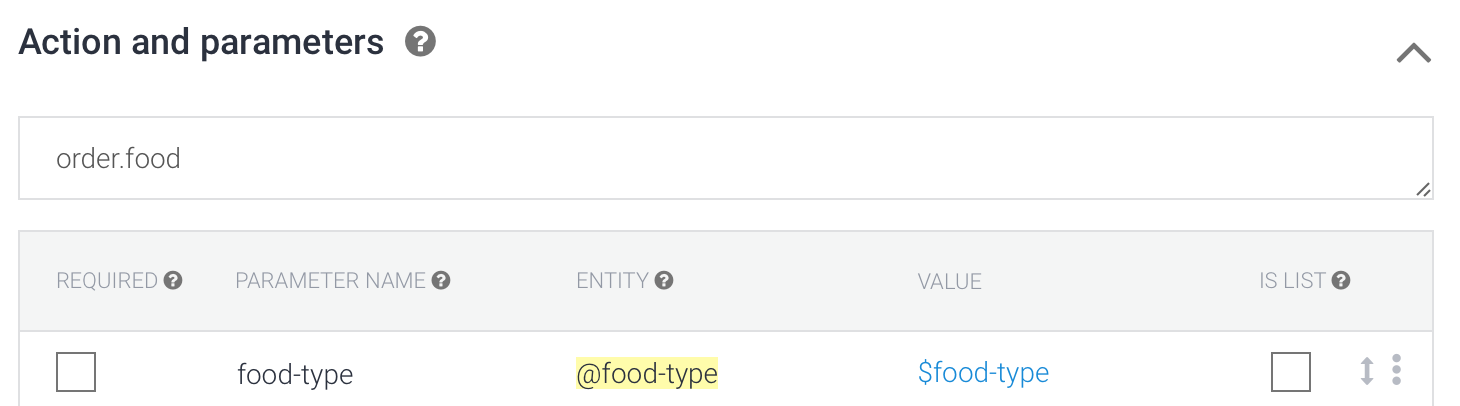
\includegraphics[width=0.9\textwidth]{parameter-table}\label{fig:parameter-table}
	\caption{The parameter table of an intent}
\end{figure}

\subsection{Events}

\subsection{Dialogs}

\subsection{Fulfillment}